% Options for packages loaded elsewhere
\PassOptionsToPackage{unicode}{hyperref}
\PassOptionsToPackage{hyphens}{url}
%
\documentclass[
]{article}
\usepackage{amsmath,amssymb}
\usepackage{iftex}
\ifPDFTeX
  \usepackage[T1]{fontenc}
  \usepackage[utf8]{inputenc}
  \usepackage{textcomp} % provide euro and other symbols
\else % if luatex or xetex
  \usepackage{unicode-math} % this also loads fontspec
  \defaultfontfeatures{Scale=MatchLowercase}
  \defaultfontfeatures[\rmfamily]{Ligatures=TeX,Scale=1}
\fi
\usepackage{lmodern}
\ifPDFTeX\else
  % xetex/luatex font selection
\fi
% Use upquote if available, for straight quotes in verbatim environments
\IfFileExists{upquote.sty}{\usepackage{upquote}}{}
\IfFileExists{microtype.sty}{% use microtype if available
  \usepackage[]{microtype}
  \UseMicrotypeSet[protrusion]{basicmath} % disable protrusion for tt fonts
}{}
\makeatletter
\@ifundefined{KOMAClassName}{% if non-KOMA class
  \IfFileExists{parskip.sty}{%
    \usepackage{parskip}
  }{% else
    \setlength{\parindent}{0pt}
    \setlength{\parskip}{6pt plus 2pt minus 1pt}}
}{% if KOMA class
  \KOMAoptions{parskip=half}}
\makeatother
\usepackage{xcolor}
\usepackage[margin=1in]{geometry}
\usepackage{color}
\usepackage{fancyvrb}
\newcommand{\VerbBar}{|}
\newcommand{\VERB}{\Verb[commandchars=\\\{\}]}
\DefineVerbatimEnvironment{Highlighting}{Verbatim}{commandchars=\\\{\}}
% Add ',fontsize=\small' for more characters per line
\usepackage{framed}
\definecolor{shadecolor}{RGB}{248,248,248}
\newenvironment{Shaded}{\begin{snugshade}}{\end{snugshade}}
\newcommand{\AlertTok}[1]{\textcolor[rgb]{0.94,0.16,0.16}{#1}}
\newcommand{\AnnotationTok}[1]{\textcolor[rgb]{0.56,0.35,0.01}{\textbf{\textit{#1}}}}
\newcommand{\AttributeTok}[1]{\textcolor[rgb]{0.13,0.29,0.53}{#1}}
\newcommand{\BaseNTok}[1]{\textcolor[rgb]{0.00,0.00,0.81}{#1}}
\newcommand{\BuiltInTok}[1]{#1}
\newcommand{\CharTok}[1]{\textcolor[rgb]{0.31,0.60,0.02}{#1}}
\newcommand{\CommentTok}[1]{\textcolor[rgb]{0.56,0.35,0.01}{\textit{#1}}}
\newcommand{\CommentVarTok}[1]{\textcolor[rgb]{0.56,0.35,0.01}{\textbf{\textit{#1}}}}
\newcommand{\ConstantTok}[1]{\textcolor[rgb]{0.56,0.35,0.01}{#1}}
\newcommand{\ControlFlowTok}[1]{\textcolor[rgb]{0.13,0.29,0.53}{\textbf{#1}}}
\newcommand{\DataTypeTok}[1]{\textcolor[rgb]{0.13,0.29,0.53}{#1}}
\newcommand{\DecValTok}[1]{\textcolor[rgb]{0.00,0.00,0.81}{#1}}
\newcommand{\DocumentationTok}[1]{\textcolor[rgb]{0.56,0.35,0.01}{\textbf{\textit{#1}}}}
\newcommand{\ErrorTok}[1]{\textcolor[rgb]{0.64,0.00,0.00}{\textbf{#1}}}
\newcommand{\ExtensionTok}[1]{#1}
\newcommand{\FloatTok}[1]{\textcolor[rgb]{0.00,0.00,0.81}{#1}}
\newcommand{\FunctionTok}[1]{\textcolor[rgb]{0.13,0.29,0.53}{\textbf{#1}}}
\newcommand{\ImportTok}[1]{#1}
\newcommand{\InformationTok}[1]{\textcolor[rgb]{0.56,0.35,0.01}{\textbf{\textit{#1}}}}
\newcommand{\KeywordTok}[1]{\textcolor[rgb]{0.13,0.29,0.53}{\textbf{#1}}}
\newcommand{\NormalTok}[1]{#1}
\newcommand{\OperatorTok}[1]{\textcolor[rgb]{0.81,0.36,0.00}{\textbf{#1}}}
\newcommand{\OtherTok}[1]{\textcolor[rgb]{0.56,0.35,0.01}{#1}}
\newcommand{\PreprocessorTok}[1]{\textcolor[rgb]{0.56,0.35,0.01}{\textit{#1}}}
\newcommand{\RegionMarkerTok}[1]{#1}
\newcommand{\SpecialCharTok}[1]{\textcolor[rgb]{0.81,0.36,0.00}{\textbf{#1}}}
\newcommand{\SpecialStringTok}[1]{\textcolor[rgb]{0.31,0.60,0.02}{#1}}
\newcommand{\StringTok}[1]{\textcolor[rgb]{0.31,0.60,0.02}{#1}}
\newcommand{\VariableTok}[1]{\textcolor[rgb]{0.00,0.00,0.00}{#1}}
\newcommand{\VerbatimStringTok}[1]{\textcolor[rgb]{0.31,0.60,0.02}{#1}}
\newcommand{\WarningTok}[1]{\textcolor[rgb]{0.56,0.35,0.01}{\textbf{\textit{#1}}}}
\usepackage{graphicx}
\makeatletter
\def\maxwidth{\ifdim\Gin@nat@width>\linewidth\linewidth\else\Gin@nat@width\fi}
\def\maxheight{\ifdim\Gin@nat@height>\textheight\textheight\else\Gin@nat@height\fi}
\makeatother
% Scale images if necessary, so that they will not overflow the page
% margins by default, and it is still possible to overwrite the defaults
% using explicit options in \includegraphics[width, height, ...]{}
\setkeys{Gin}{width=\maxwidth,height=\maxheight,keepaspectratio}
% Set default figure placement to htbp
\makeatletter
\def\fps@figure{htbp}
\makeatother
\setlength{\emergencystretch}{3em} % prevent overfull lines
\providecommand{\tightlist}{%
  \setlength{\itemsep}{0pt}\setlength{\parskip}{0pt}}
\setcounter{secnumdepth}{-\maxdimen} % remove section numbering
\ifLuaTeX
  \usepackage{selnolig}  % disable illegal ligatures
\fi
\usepackage{bookmark}
\IfFileExists{xurl.sty}{\usepackage{xurl}}{} % add URL line breaks if available
\urlstyle{same}
\hypersetup{
  pdftitle={Differential Gene Expression Analysis},
  pdfauthor={Zilan Wen},
  hidelinks,
  pdfcreator={LaTeX via pandoc}}

\title{Differential Gene Expression Analysis}
\author{Zilan Wen}
\date{2024-05-13}

\begin{document}
\maketitle

\section{1 Install R package, RStudio, directory set-up,
GitHub}\label{install-r-package-rstudio-directory-set-up-github}

\subsection{1.1 Install R and RStudio}\label{install-r-and-rstudio}

Install R and install RStudio on your own laptop or owned computer
\url{https://posit.co/download/rstudio-desktop/} based on your operating
system, available for Linux, MacOS, and Windows Install R and install
RStudio on the University computers: go to Start manu --\textgreater{}
Software Center --\textgreater{} search for RStudio, and R for Windows.
The current version of R in the computers here is 4.3.2

\subsection{1.2 Differential expression analysis (DEA) work directory
setting
up}\label{differential-expression-analysis-dea-work-directory-setting-up}

Open up RStudio and setting up a new project for DEA analysis

1.Go to the \texttt{File} menu and select \texttt{New\ Project}.

2.In the \texttt{New\ Project} window, choose \texttt{New\ Directory}.
Then, choose \texttt{New\ Project}. Name your new directory
\texttt{RNA\_seq\_DEA} and then ``Create the project as subdirectory
of:'' the Desktop or \texttt{OneDrive\ -\ University\ of\ Helsinki} (or
location of your choice).

3.The new project should automatically open in RStudio.\\

\includegraphics[width=0.5\textwidth,height=\textheight]{C:/Users/timoi/OneDrive - University of Helsinki/ZilanWen Github/RNA-seq_Differential-Gene-Expression-Analysis/image/Create_RStudio_Project.gif}\\

To check whether or not you are in the correct working directory, use
getwd(). The path Desktop/RNA\_seq\_DEA should be returned to you in the
console.

\begin{Shaded}
\begin{Highlighting}[]
\FunctionTok{getwd}\NormalTok{()}
\end{Highlighting}
\end{Shaded}

\begin{verbatim}
## [1] "C:/Users/timoi/OneDrive - University of Helsinki/ZilanWen Github/RNA-seq_Differential-Gene-Expression-Analysis"
\end{verbatim}

To get the location of working directory For example: At Desktop, build
a folder At RStudio --\textgreater{} Session --\textgreater{} Set
Working Directory --\textgreater{} Choose Directory --\textgreater{}
Desktop --\textgreater{} RNA-seq\_DEA

or use code below:

\begin{Shaded}
\begin{Highlighting}[]
\FunctionTok{setwd}\NormalTok{(}\StringTok{"C:/Users/username/Desktop/RNA{-}seq\_DEA"}\NormalTok{)}
\end{Highlighting}
\end{Shaded}

Check the current R version. The current R version is R-4.4.0

\begin{Shaded}
\begin{Highlighting}[]
\FunctionTok{R.Version}\NormalTok{()}\CommentTok{\#the code in the code chunk will not be run.}
\end{Highlighting}
\end{Shaded}

Within your working directory use the New folder button in the bottom
right panel to create two new directories \texttt{data} and
\texttt{results}.

Now we need to download the files from \texttt{Moodle} and the data list
which looks like below\\
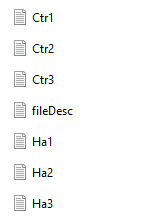
\includegraphics[width=0.15\textwidth,height=\textheight]{C:/Users/timoi/OneDrive - University of Helsinki/ZilanWen Github/RNA-seq_Differential-Gene-Expression-Analysis/image/data.png}
Then we go to the File menu and select New File, then select R Script.
This should open up a script editor in the top left hand corner. This is
where we will be typing and saving all commands required for this
analysis. Now save the file as DEA\_script.R. When finished your working
directory should now look similar to this:\\
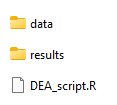
\includegraphics{C:/Users/timoi/OneDrive - University of Helsinki/ZilanWen Github/RNA-seq_Differential-Gene-Expression-Analysis/image/dir.png}
\texttt{data} for the original data, \texttt{results} for generated
files and figures.

\subsection{1.3 GitHub (optional)}\label{github-optional}

GitHub is an online software development platform. It's used for
storing, tracking, and collaborating on software projects. It makes it
easy for developers to share code files and collaborate with fellow
developers on open-source projects.

\begin{itemize}
\item
  \textbf{Set up your GitHub}: Go here \url{https://github.com/}, log in
  or sign up with your email.
\item
  \textbf{Create your repository}: Repository is the project you can
  create which is on the top left of your GitHub home page.To create a
  new repository, you can click the green button \texttt{New}, then name
  the new repository.Choose Public or Private, and initialize this
  repository with add a README file. Next Click
  \texttt{Create\ repository}. The list of repositories is on your
  Github home page.
\item
  \textbf{Use the Github desktop version}: We are going to download and
  upload by commiting changes from our local files to the cloud. Go to
  GitHub Desktop\url{https://desktop.github.com/}, download based on
  your operating system. Then go to sign in with your GitHub account.Go
  back to your GitHUb repository, and click open with Github Desktop\\
  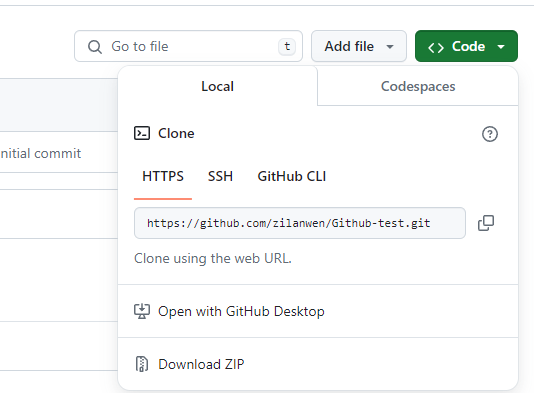
\includegraphics[width=0.5\textwidth,height=\textheight]{C:/Users/timoi/OneDrive - University of Helsinki/ZilanWen Github/RNA-seq_Differential-Gene-Expression-Analysis/image/Github1.png}
\item
  \textbf{Clone a repository and connect repository to local files} In
  local path, choose where we want to save the repository in our local
  computer.click \texttt{Clone}. Now we have cloned the repository that
  we created on GitHub and we have connected it to the GitHub desktop
  application.\\
  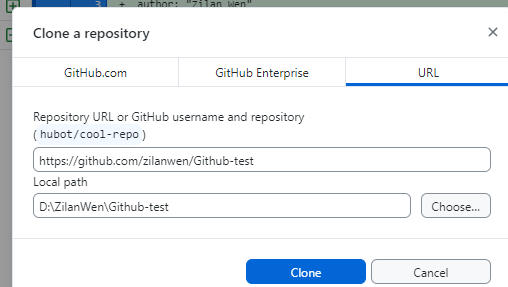
\includegraphics[width=0.5\textwidth,height=\textheight]{C:/Users/timoi/OneDrive - University of Helsinki/ZilanWen Github/RNA-seq_Differential-Gene-Expression-Analysis/image/Github2.png}
\item
  \textbf{upload local files to GitHub cloud} Any changes and updated
  files can be uploaded to GitHUb cloud though GitHub Desktop.Atfter
  change files, go back to GitHub Desktop and navigate the corresponding
  repository, you will have the changes listed on the top left. We now
  give the change a title such as `11' in
  the\texttt{summary\ (required)}box and click \texttt{Commit\ to\ main}
  on the bottom left, Then on the right, we can push comments to the
  origin remote by clicking \texttt{Push\ origin}.\\
  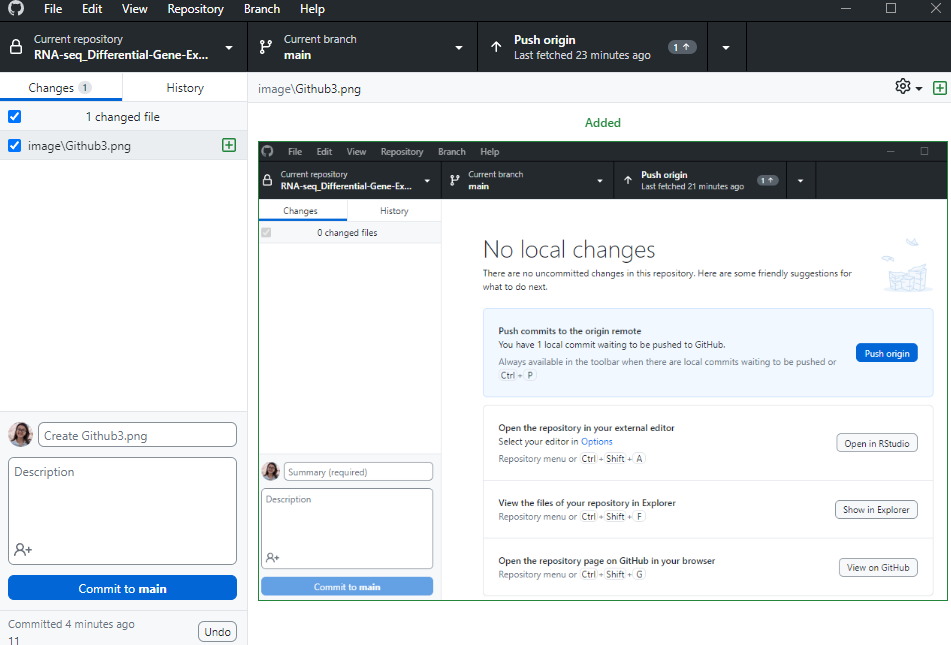
\includegraphics[width=0.5\textwidth,height=\textheight]{C:/Users/timoi/OneDrive - University of Helsinki/ZilanWen Github/RNA-seq_Differential-Gene-Expression-Analysis/image/Github3.png}
\item
  \textbf{Clone a repository from other GitHUb accounts} Forking a
  repository can make a copy of a repository from other account to your
  account.\\
\end{itemize}

\begin{figure}
\centering

\includegraphics[width=0.5\textwidth,height=\textheight]{C:/Users/timoi/OneDrive - University of Helsinki/ZilanWen Github/RNA-seq_Differential-Gene-Expression-Analysis/image/Github5.png}
\caption{3}
\end{figure}

\section{2 Count normalization}\label{count-normalization}

Created on 14.05.2024\\
@author: Zilan Wen\\
Email:
\href{mailto:zilan.wen@helsinki.fi}{\nolinkurl{zilan.wen@helsinki.fi}}

\subsection{2.1 Normalization Overview}\label{normalization-overview}

The first step in the DE analysis workflow is count normalization, which
is necessary to make accurate comparisons of gene expression between
samples.

The main factors often considered during normalization are:

\begin{itemize}
\tightlist
\item
  sequencing depth or coverage.
\end{itemize}

\begin{figure}
\centering
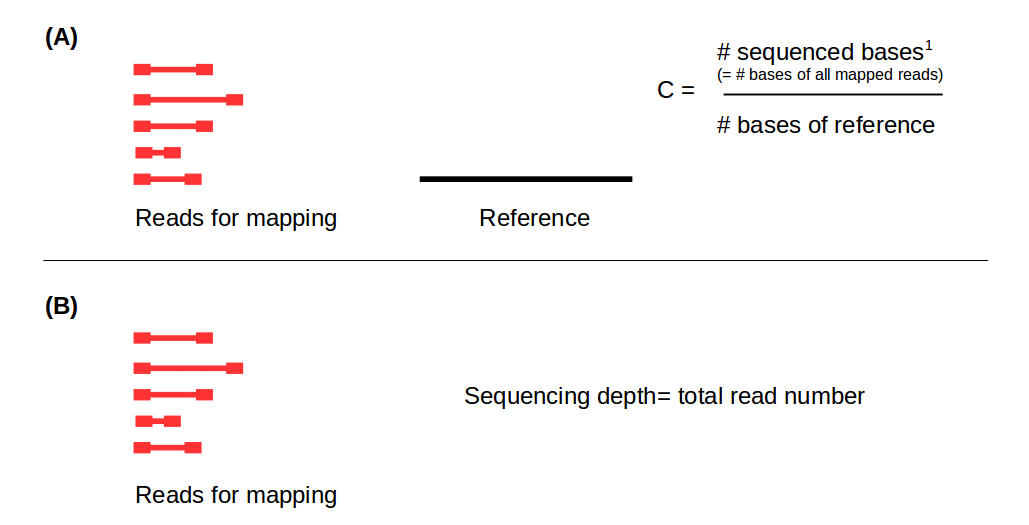
\includegraphics[width=0.5\textwidth,height=\textheight]{C:/Users/timoi/OneDrive - University of Helsinki/ZilanWen Github/RNA-seq_Differential-Gene-Expression-Analysis/image/Github4.png}
\caption{4}
\end{figure}

\begin{itemize}
\item
  Gene length
\item
  RNA composition
\end{itemize}

These three factors have been described very well in {[}DEG workshop
Salmon{]}
(\url{https://github.com/hbctraining/DGE_workshop_salmon/blob/master/lessons/02_DGE_count_normalization.md})

\section{2.1.1 Common normalization
methods}\label{common-normalization-methods}

\begin{itemize}
\item
  \texttt{CPM} \emph{counts per million} counts scaled by total number
  of reads.
\item
  \texttt{TPM}\emph{transcripts per kilobase million} counts per length
  of transcript (kb) per million reads mapped.
\item
  \texttt{RPKM} or \texttt{RKPM} \emph{reads/fragments per kilobase of
  exon per million reads / fragments mapped} similar to TPM.
  \texttt{DESeq2\textquotesingle{}s\ median\ of\ ratios} counts divided
  by sample-specific size factors determined by median ratio of gene
  counts relative to geometric mean per gene.
\item
  \texttt{EdgeR\textquotesingle{}s\ trimmed\ mean\ of\ M\ values\ (TMM)}
  uses a weighted trimmed mean of the log expression ratios between
  samples.
\end{itemize}

The differences between RPKM, FPKM and TPM are explained clearly by
\href{https://www.rna-seqblog.com/rpkm-fpkm-and-tpm-clearly-explained/}{SatQuest
video}

\section{2.1.2 DESeq2-normalized counts: Median of ratios
method}\label{deseq2-normalized-counts-median-of-ratios-method}

This method is explained clearly in
\href{https://github.com/hbctraining/DGE_workshop_salmon/blob/master/lessons/02_DGE_count_normalization.md}{DEG\_workshop\_salmon}
Since tools for differential expression analysis are comparing the
counts between sample groups for the same gene, gene length does not
need to be accounted for by the tool. However,
\texttt{sequencing\ depth} and \texttt{RNA\ composition} need to be
taken into account.

\subsection{2.2 Count normalization of our dataset with
DESeq2}\label{count-normalization-of-our-dataset-with-deseq2}

For transcriptome study, RNA samples which are isolated from control
samples and treatment samples are sent to sequencing company. The
following steps are :

\begin{itemize}
\item
  RNA-seq with a sequencing depth of 10-30 M reads per library (at least
  3 biological replicates per sample)
\item
  Aligning or mapping the quality-filtered sequenced reads to respective
  genome (e.g.~HISAT2 or STAR or Bowtie2).
\item
  Quantifying reads that are mapped to genes or transcripts (e.g.HTseq)
\item
  Gene differential expression analysis
\item
  Functional analysis such as enrichment of known biological functions,
  interactions, or pathways
\end{itemize}

\textbf{RNA samples} \emph{Heterobasidion annosum} is a forest pathogen
which can cause root and stem rot disease on Scots pine and Norway
spruce. In this experiment, two-month old Scots pine plants were
inoculated with H. annosum. After one month infection, total RNA was
extracted from Scots pine roots. Control plants were fungus-free. We
have three biological replicates for each treatment. The treatment
samples are \texttt{Ha1},\texttt{Ha2}, \texttt{Ha3} and the control
samples are \texttt{Ctr1}, \texttt{Ctr2}, \texttt{Ctr3}. Since genome of
Scots pine is not available, we align reads to \emph{Pinus taeda} genome
which can be found in plantgenie \url{https://plantgenie.org/}.

In this tutorial we start with raw reads count ´.txt´ files, normalize
the counts using DESeq2.This requires a few steps:

\begin{itemize}
\tightlist
\item
  \begin{enumerate}
  \def\labelenumi{\arabic{enumi}.}
  \tightlist
  \item
    Install packages \texttt{DESeq2}, \texttt{EdgeR}
  \end{enumerate}
\item
  \begin{enumerate}
  \def\labelenumi{\arabic{enumi}.}
  \setcounter{enumi}{1}
  \tightlist
  \item
    Build a file description \texttt{fileDesc.txt} file for all
    \texttt{.txt} files about counts matrix,including file path,
    inoculation, and description.
  \end{enumerate}
\item
  \begin{enumerate}
  \def\labelenumi{\arabic{enumi}.}
  \setcounter{enumi}{2}
  \tightlist
  \item
    Read data files.
  \end{enumerate}
\item
  \begin{enumerate}
  \def\labelenumi{\arabic{enumi}.}
  \setcounter{enumi}{3}
  \tightlist
  \item
    Build \texttt{meta} data. \texttt{meta} file is similar to
    \texttt{filedesc}, bnut we use meta for create \texttt{DESeqDataset}
    object. Ensure the row names of the metadata dataframe are present
    and in the same order as the column names of the counts data frame.
  \end{enumerate}
\item
  \begin{enumerate}
  \def\labelenumi{\arabic{enumi}.}
  \setcounter{enumi}{4}
  \tightlist
  \item
    Create \texttt{DESeqDataset} object
  \end{enumerate}
\item
  \begin{enumerate}
  \def\labelenumi{\arabic{enumi}.}
  \setcounter{enumi}{5}
  \tightlist
  \item
    Generate size factors
  \end{enumerate}
\item
  \begin{enumerate}
  \def\labelenumi{\arabic{enumi}.}
  \setcounter{enumi}{6}
  \tightlist
  \item
    Generate the normalized counts
  \end{enumerate}
\end{itemize}

\subsubsection{2.2.1 Install packages}\label{install-packages}

Install \texttt{DESeq2} package

\begin{Shaded}
\begin{Highlighting}[]
\ControlFlowTok{if}\NormalTok{ (}\SpecialCharTok{!}\FunctionTok{require}\NormalTok{(}\StringTok{"BiocManager"}\NormalTok{, }\AttributeTok{quietly =} \ConstantTok{TRUE}\NormalTok{))}
    \FunctionTok{install.packages}\NormalTok{(}\StringTok{"BiocManager"}\NormalTok{)}

\NormalTok{BiocManager}\SpecialCharTok{::}\FunctionTok{install}\NormalTok{(}\StringTok{"DESeq2"}\NormalTok{)}
\end{Highlighting}
\end{Shaded}

We need to install \texttt{EdgeR} package because we need the readDGE
function here.

\begin{Shaded}
\begin{Highlighting}[]
\ControlFlowTok{if}\NormalTok{ (}\SpecialCharTok{!}\FunctionTok{require}\NormalTok{(}\StringTok{"BiocManager"}\NormalTok{, }\AttributeTok{quietly =} \ConstantTok{TRUE}\NormalTok{))}
    \FunctionTok{install.packages}\NormalTok{(}\StringTok{"BiocManager"}\NormalTok{)}

\NormalTok{BiocManager}\SpecialCharTok{::}\FunctionTok{install}\NormalTok{(}\StringTok{"edgeR"}\NormalTok{)}
\end{Highlighting}
\end{Shaded}

\subsubsection{2.2.2 Build a file
description}\label{build-a-file-description}

Here the file description called \texttt{fileDesc} is already build and
save in \texttt{data} folder. We will use it for reading a list of
seperated files.

\subsubsection{2.2.3 Read data files}\label{read-data-files}

Set to the current work directory

\begin{Shaded}
\begin{Highlighting}[]
\FunctionTok{setwd}\NormalTok{(}\StringTok{\textquotesingle{}C:/Users/timoi/OneDrive {-} University of Helsinki/ZilanWen Github/RNA{-}seq\_Differential{-}Gene{-}Expression{-}Analysis\textquotesingle{}}\NormalTok{)}
\end{Highlighting}
\end{Shaded}

Now we start to read raw data

\begin{Shaded}
\begin{Highlighting}[]
\NormalTok{Coinfection.targets}\OtherTok{\textless{}{-}}\FunctionTok{read.delim}\NormalTok{(}\StringTok{"./data/fileDesc.txt"}\NormalTok{)}
\end{Highlighting}
\end{Shaded}

change the rawnames of the dataframe \texttt{Coinfection.targets}, later
on we don't need to rename column names.

\begin{Shaded}
\begin{Highlighting}[]
\FunctionTok{rownames}\NormalTok{(Coinfection.targets)}\OtherTok{\textless{}{-}}\FunctionTok{c}\NormalTok{(}\StringTok{"Ha1"}\NormalTok{,}\StringTok{"Ha2"}\NormalTok{,}\StringTok{"Ha3"}\NormalTok{,}\StringTok{"Ctr1"}\NormalTok{,}\StringTok{"Ctr2"}\NormalTok{,}\StringTok{"Ctr3"}\NormalTok{)}
\end{Highlighting}
\end{Shaded}

load the packege \texttt{edgeR}

\begin{Shaded}
\begin{Highlighting}[]
\FunctionTok{library}\NormalTok{(edgeR)}
\end{Highlighting}
\end{Shaded}

\begin{verbatim}
## Loading required package: limma
\end{verbatim}

read the six \texttt{.txt} files listed in \texttt{Coinfection.targets}.

\begin{Shaded}
\begin{Highlighting}[]
\NormalTok{Coinfection.orig }\OtherTok{\textless{}{-}} \FunctionTok{readDGE}\NormalTok{(Coinfection.targets, }\AttributeTok{header=}\NormalTok{F)}
\end{Highlighting}
\end{Shaded}

check the dimension of the data set

\begin{Shaded}
\begin{Highlighting}[]
\FunctionTok{dim}\NormalTok{(Coinfection.orig)}
\end{Highlighting}
\end{Shaded}

\begin{verbatim}
## [1] 51751     6
\end{verbatim}

chreck the first 6 rows of the data

\begin{Shaded}
\begin{Highlighting}[]
\FunctionTok{head}\NormalTok{(Coinfection.orig)}
\end{Highlighting}
\end{Shaded}

\begin{verbatim}
## An object of class "DGEList"
## $samples
##           files.path inoculation         description           files group
## Ha1   ./data/Ha1.txt          Ha H.annosum infection  ./data/Ha1.txt     1
## Ha2   ./data/Ha2.txt          Ha H.annosum infection  ./data/Ha2.txt     1
## Ha3   ./data/Ha3.txt          Ha H.annosum infection  ./data/Ha3.txt     1
## Ctr1 ./data/Ctr1.txt         Ctr             Control ./data/Ctr1.txt     1
## Ctr2 ./data/Ctr2.txt         Ctr             Control ./data/Ctr2.txt     1
## Ctr3 ./data/Ctr3.txt         Ctr             Control ./data/Ctr3.txt     1
##      lib.size norm.factors
## Ha1  12510293            1
## Ha2   8033676            1
## Ha3  10094630            1
## Ctr1 10763763            1
## Ctr2 10539029            1
## Ctr3 12251172            1
## 
## $counts
##             Samples
## Tags         Ha1 Ha2 Ha3 Ctr1 Ctr2 Ctr3
##   PITA_19277 274 169 195   90   80  329
##   PITA_36893   0   0   0    0    0    0
##   PITA_43071 157 101 150  128  133  127
##   PITA_31484   0   0   0    0    0    0
##   PITA_22913   0   0   0    0    0    0
##   PITA_43120  62  42  22   53   24   15
\end{verbatim}

Extact counts dataframe

\begin{Shaded}
\begin{Highlighting}[]
\NormalTok{Coinfection.rawCount }\OtherTok{\textless{}{-}}\NormalTok{ Coinfection.orig}\SpecialCharTok{$}\NormalTok{count}
\FunctionTok{dim}\NormalTok{(Coinfection.rawCount)}
\end{Highlighting}
\end{Shaded}

\begin{verbatim}
## [1] 51751     6
\end{verbatim}

\begin{Shaded}
\begin{Highlighting}[]
\FunctionTok{head}\NormalTok{(Coinfection.rawCount)}
\end{Highlighting}
\end{Shaded}

\begin{verbatim}
##             Samples
## Tags         Ha1 Ha2 Ha3 Ctr1 Ctr2 Ctr3
##   PITA_19277 274 169 195   90   80  329
##   PITA_36893   0   0   0    0    0    0
##   PITA_43071 157 101 150  128  133  127
##   PITA_31484   0   0   0    0    0    0
##   PITA_22913   0   0   0    0    0    0
##   PITA_43120  62  42  22   53   24   15
\end{verbatim}

\subsubsection{2.2.4 Build meta data}\label{build-meta-data}

We define \texttt{sampletype}: we only have two types of samples,
Control and Ha-infection

\begin{Shaded}
\begin{Highlighting}[]
\NormalTok{sampletype }\OtherTok{\textless{}{-}} \FunctionTok{factor}\NormalTok{(}\FunctionTok{c}\NormalTok{(}\FunctionTok{rep}\NormalTok{(}\StringTok{"Ha"}\NormalTok{,}\DecValTok{3}\NormalTok{), }\FunctionTok{rep}\NormalTok{(}\StringTok{"Ctr"}\NormalTok{, }\DecValTok{3}\NormalTok{)))}
\end{Highlighting}
\end{Shaded}

Build meta data frame

\begin{Shaded}
\begin{Highlighting}[]
\NormalTok{meta }\OtherTok{\textless{}{-}} \FunctionTok{data.frame}\NormalTok{(sampletype, }\AttributeTok{row.names =} \FunctionTok{colnames}\NormalTok{(Coinfection.orig}\SpecialCharTok{$}\NormalTok{count))}
\end{Highlighting}
\end{Shaded}

check the column name of counts dataframe

\begin{Shaded}
\begin{Highlighting}[]
\FunctionTok{colnames}\NormalTok{(Coinfection.orig}\SpecialCharTok{$}\NormalTok{count)}
\end{Highlighting}
\end{Shaded}

\begin{verbatim}
## [1] "Ha1"  "Ha2"  "Ha3"  "Ctr1" "Ctr2" "Ctr3"
\end{verbatim}

check the rowname of meta dataframe

\begin{Shaded}
\begin{Highlighting}[]
\FunctionTok{rownames}\NormalTok{(meta)}
\end{Highlighting}
\end{Shaded}

\begin{verbatim}
## [1] "Ha1"  "Ha2"  "Ha3"  "Ctr1" "Ctr2" "Ctr3"
\end{verbatim}

Check that sample names match in both files

\begin{Shaded}
\begin{Highlighting}[]
\FunctionTok{all}\NormalTok{(}\FunctionTok{colnames}\NormalTok{(Coinfection.orig}\SpecialCharTok{$}\NormalTok{count) }\SpecialCharTok{\%in\%} \FunctionTok{rownames}\NormalTok{(meta))}
\end{Highlighting}
\end{Shaded}

\begin{verbatim}
## [1] TRUE
\end{verbatim}

\subsubsection{\texorpdfstring{2.2.5 Create \texttt{DESeqDataset}
object}{2.2.5 Create DESeqDataset object}}\label{create-deseqdataset-object}

load the package \texttt{DESeq2} Create DESEq2 dataset \texttt{dds}

\begin{Shaded}
\begin{Highlighting}[]
\FunctionTok{library}\NormalTok{(DESeq2)}
\NormalTok{dds }\OtherTok{\textless{}{-}} \FunctionTok{DESeqDataSetFromMatrix}\NormalTok{(Coinfection.orig, }\AttributeTok{colData =}\NormalTok{ meta, }\AttributeTok{design =} \SpecialCharTok{\textasciitilde{}}\NormalTok{ sampletype)}
\end{Highlighting}
\end{Shaded}

If you want to view dds, you can use the code:

\begin{Shaded}
\begin{Highlighting}[]
\FunctionTok{head}\NormalTok{(}\FunctionTok{counts}\NormalTok{(dds))}
\end{Highlighting}
\end{Shaded}

\begin{verbatim}
##             Samples
## Tags         Ha1 Ha2 Ha3 Ctr1 Ctr2 Ctr3
##   PITA_19277 274 169 195   90   80  329
##   PITA_36893   0   0   0    0    0    0
##   PITA_43071 157 101 150  128  133  127
##   PITA_31484   0   0   0    0    0    0
##   PITA_22913   0   0   0    0    0    0
##   PITA_43120  62  42  22   53   24   15
\end{verbatim}

\subsubsection{2.2.6 Generate size factors}\label{generate-size-factors}

To perform the median of ratios method of normalization, DESeq2 has a
single estimateSizeFactors() function that will generate size factors.

\begin{Shaded}
\begin{Highlighting}[]
\NormalTok{dds }\OtherTok{\textless{}{-}} \FunctionTok{estimateSizeFactors}\NormalTok{(dds)}
\end{Highlighting}
\end{Shaded}

take a look at the normalization factor applied to each sample

\begin{Shaded}
\begin{Highlighting}[]
\FunctionTok{sizeFactors}\NormalTok{(dds)}
\end{Highlighting}
\end{Shaded}

\begin{verbatim}
##       Ha1       Ha2       Ha3      Ctr1      Ctr2      Ctr3 
## 1.1734464 0.7897579 0.9805609 1.0611942 0.9794690 1.1512821
\end{verbatim}

\subsubsection{2.2.7 Generate the normalized
counts}\label{generate-the-normalized-counts}

Now, to retrieve the normalized counts matrix from dds, we use the
counts() function and add the argument normalized=TRUE.

\begin{Shaded}
\begin{Highlighting}[]
\NormalTok{normalized\_counts }\OtherTok{\textless{}{-}} \FunctionTok{counts}\NormalTok{(dds, }\AttributeTok{normalized=}\ConstantTok{TRUE}\NormalTok{)}
\end{Highlighting}
\end{Shaded}

Save the \texttt{normalized\_counts}into results to your local path.

\begin{Shaded}
\begin{Highlighting}[]
\FunctionTok{write.csv}\NormalTok{(normalized\_counts, }\AttributeTok{file=}\StringTok{"./results/coinfection\_normalized\_counts\_DESeq2.csv"}\NormalTok{)}
\end{Highlighting}
\end{Shaded}

\section{3 Sample-level quality
Control}\label{sample-level-quality-control}

\subsection{3.1 Principal Component Analysis
(PCA)}\label{principal-component-analysis-pca}

\subsubsection{3.1.1 PCA overview}\label{pca-overview}

A useful initial step in an RNA-seq analysis is often to assess overall
similarity between samples:

\begin{itemize}
\item
  Which samples are similar to each other, which are different?
\item
  Does this fit to the expectation from the experiment's design?
\item
  What are the major sources of variation in the dataset?
\end{itemize}

To explore the similarity of our samples, we will be performing
sample-level QC using Principal Component Analysis (PCA) and
hierarchical clustering methods. These methods/tools allow us to check
how well similar the replicates are to each other (clustering) and to
make sure that the experimental condition is the major source of
variation in the data. Sample-level QC can also help identify any
samples behaving like outliers; we can further explore any potential
outliers to determine whether they need to be removed prior to DE
analysis.

These unsupervised clustering methods are run using log2 transformed
normalized counts. The log2 transformation improves the
distances/clustering for visualization. Instead of using an ordinary
log2 transform, we will be using regularized log transform (rlog), to
avoid any bias from the abundance of low-count genes; Note1 below
explains this in more detail.

For more details, please go to
\href{https://github.com/zilanwen/DGE_workshop_salmon_online/blob/master/lessons/03_DGE_QC_analysis.md}{DEG
workshop Salmon}

\subsubsection{3.1.2 Using our dataset for
PCA}\label{using-our-dataset-for-pca}

\begin{itemize}
\tightlist
\item
  \textbf{Transform normalized counts for the dataset}
\end{itemize}

To improve the distances/clustering for the PCA and heirarchical
clustering visualization methods, we need to moderate the variance
across the mean by applying the rlog transformation to the normalized
counts.

Transform counts for data visualization

\begin{Shaded}
\begin{Highlighting}[]
\NormalTok{rld }\OtherTok{\textless{}{-}} \FunctionTok{rlog}\NormalTok{(dds, }\AttributeTok{blind=}\ConstantTok{TRUE}\NormalTok{)}
\end{Highlighting}
\end{Shaded}

The \texttt{blind=TRUE} argument is to make sure that the
\texttt{rlog()} function does not take our sample groups into account -
i.e.~does the transformation in an unbiased manner. When performing
quality assessment, it is important to include this option. The
\href{https://bioconductor.org/packages/devel/bioc/vignettes/DESeq2/inst/doc/DESeq2.html\#blind-dispersion-estimation}{DESeq2
vignette} has more details about this.

The \texttt{rlog()} function returns a \texttt{DESeqTransform} object,
another type of DESeq-specific object. The reason you don't just get a
matrix of transformed values is because all of the parameters (i.e.~size
factors) that went into computing the rlog transform are stored in that
object. We use this object to plot the PCA and heirarchical clustering
figures for quality assessment.

\begin{itemize}
\tightlist
\item
  \textbf{start with PCA}
\end{itemize}

The function plotPCA() requires two arguments as input: a DESeqTransform
object and the ``intgroup'' (interesting group), i.e.~the name of the
column in our metadata that has information about the experimental
sample groups.

\begin{Shaded}
\begin{Highlighting}[]
\FunctionTok{plotPCA}\NormalTok{(rld, }\AttributeTok{intgroup=}\StringTok{"sampletype"}\NormalTok{)}
\end{Highlighting}
\end{Shaded}

\begin{verbatim}
## using ntop=500 top features by variance
\end{verbatim}

\includegraphics{index_files/figure-latex/unnamed-chunk-26-1.pdf} If we
want to save PDF file on own computer:

\begin{Shaded}
\begin{Highlighting}[]
\FunctionTok{pdf}\NormalTok{(}\StringTok{"./results/PlotPCA\_dds.pdf"}\NormalTok{)}
\FunctionTok{plotPCA}\NormalTok{(rld, }\AttributeTok{intgroup=}\StringTok{"sampletype"}\NormalTok{)}
\FunctionTok{dev.off}\NormalTok{()}
\end{Highlighting}
\end{Shaded}

\begin{itemize}
\item
  \textbf{Exercise}:
\item
  \begin{enumerate}
  \def\labelenumi{\arabic{enumi}.}
  \tightlist
  \item
    What does the above plot tell you about the similarity of samples?
  \end{enumerate}
\item
  \begin{enumerate}
  \def\labelenumi{\arabic{enumi}.}
  \setcounter{enumi}{1}
  \tightlist
  \item
    Does it fit the expectation from the experimental design?
  \end{enumerate}
\item
  \begin{enumerate}
  \def\labelenumi{\arabic{enumi}.}
  \setcounter{enumi}{2}
  \tightlist
  \item
    What do you think the \%variance information (in the axes titles)
    tell you about the data in the context of the PCA?
  \end{enumerate}
\end{itemize}

\subsection{3.2 Hierarchical Clustering
Heatmap}\label{hierarchical-clustering-heatmap}

Similar to PCA, hierarchical clustering is another, complementary,
method for identifying strong patterns in a dataset and potential
outliers. The heatmap displays the \textbf{correlation of gene
expression for all pairwise combinations of samples} in the dataset.
Since the majority of genes are not differentially expressed, samples
generally have high correlations with each other (values higher than
0.80). Samples below 0.80 may indicate an outlier in your data and/or
sample contamination.

There is no built-in function in DESeq2 for plotting the heatmap for
diplaying the pairwise correlation between all the samples and the
hierarchical clustering information; we will use the \texttt{pheatmap()}
function from the \texttt{pheatmap} package. This function cannot use
the \texttt{DESeqTransform} object as input, but requires a matrix or
dataframe. So, the first thing to do is retrieve that information from
the \texttt{rld} object using a function called \texttt{assay()} (from
the \texttt{SummarizedExperiment} package) that converts the data in a
\texttt{DESeqTransform} object to a simple 2-dimensional data structure
(a matrix in this case).

Extract the rlog matrix from the object using \texttt{assay} function
which is part of the \texttt{SummarizedExperiment} package which is a
DESeq2 dependency and is loaded with the \texttt{DESeq2} library

\begin{Shaded}
\begin{Highlighting}[]
\NormalTok{rld\_mat }\OtherTok{\textless{}{-}} \FunctionTok{assay}\NormalTok{(rld)}
\end{Highlighting}
\end{Shaded}

Next, we need to compute the pairwise correlation values for all the
samples. We can do this using the \texttt{cor()} function:

\begin{Shaded}
\begin{Highlighting}[]
\NormalTok{rld\_cor }\OtherTok{\textless{}{-}} \FunctionTok{cor}\NormalTok{(rld\_mat) }
\end{Highlighting}
\end{Shaded}

check the output of \texttt{cor()}, make note of the row names and
column names

\begin{Shaded}
\begin{Highlighting}[]
\FunctionTok{head}\NormalTok{(rld\_cor)}
\end{Highlighting}
\end{Shaded}

\begin{verbatim}
##            Ha1       Ha2       Ha3      Ctr1      Ctr2      Ctr3
## Ha1  1.0000000 0.9974935 0.9978500 0.9956639 0.9956698 0.9937710
## Ha2  0.9974935 1.0000000 0.9978706 0.9961065 0.9957914 0.9953450
## Ha3  0.9978500 0.9978706 1.0000000 0.9956039 0.9954369 0.9943809
## Ctr1 0.9956639 0.9961065 0.9956039 1.0000000 0.9967852 0.9946562
## Ctr2 0.9956698 0.9957914 0.9954369 0.9967852 1.0000000 0.9943313
## Ctr3 0.9937710 0.9953450 0.9943809 0.9946562 0.9943313 1.0000000
\end{verbatim}

We will use \texttt{meta} for annotation argument later, let's check
\texttt{meta} :

\begin{Shaded}
\begin{Highlighting}[]
\FunctionTok{head}\NormalTok{(meta)}
\end{Highlighting}
\end{Shaded}

\begin{verbatim}
##      sampletype
## Ha1          Ha
## Ha2          Ha
## Ha3          Ha
## Ctr1        Ctr
## Ctr2        Ctr
## Ctr3        Ctr
\end{verbatim}

Install \texttt{pheatmap} package and load the package

\begin{Shaded}
\begin{Highlighting}[]
\FunctionTok{install.packages}\NormalTok{(}\StringTok{"pheatmap"}\NormalTok{)}

\NormalTok{?pheatmap }\CommentTok{\# help page for pheatmap}
\end{Highlighting}
\end{Shaded}

Plot heatmap using the correlation matrix and the metadata object

\begin{Shaded}
\begin{Highlighting}[]
\FunctionTok{library}\NormalTok{(pheatmap)}
\FunctionTok{pheatmap}\NormalTok{(rld\_cor, }\AttributeTok{annotation =}\NormalTok{ meta)}
\end{Highlighting}
\end{Shaded}

\includegraphics{index_files/figure-latex/unnamed-chunk-33-1.pdf} If we
want to change color, we can try the codes below: R color in Brewer's
palettes can be available the link
\url{https://r-graph-gallery.com/38-rcolorbrewers-palettes}

pheatmap function instruction are also available {[}pheatmap{]}
(\url{https://www.rdocumentation.org/packages/pheatmap/versions/1.0.12/topics/pheatmap})

\begin{Shaded}
\begin{Highlighting}[]
\NormalTok{heat.colors }\OtherTok{\textless{}{-}}\NormalTok{ RColorBrewer}\SpecialCharTok{::}\FunctionTok{brewer.pal}\NormalTok{(}\DecValTok{6}\NormalTok{, }\StringTok{"Blues"}\NormalTok{)}
\FunctionTok{pheatmap}\NormalTok{(rld\_cor, }\AttributeTok{annotation =}\NormalTok{ meta, }\AttributeTok{color =}\NormalTok{ heat.colors, }\AttributeTok{border\_color=}\ConstantTok{NA}\NormalTok{, }\AttributeTok{fontsize =} \DecValTok{10}\NormalTok{, }
        \AttributeTok{fontsize\_row =} \DecValTok{10}\NormalTok{, }\AttributeTok{height=}\DecValTok{20}\NormalTok{)}
\end{Highlighting}
\end{Shaded}

\includegraphics{index_files/figure-latex/unnamed-chunk-34-1.pdf} If you
want to save the heatmap in local path in your computer:

\begin{Shaded}
\begin{Highlighting}[]
\FunctionTok{pdf}\NormalTok{(}\StringTok{"./results/PlotHeatmap\_dds.pdf"}\NormalTok{)}
\NormalTok{heat.colors }\OtherTok{\textless{}{-}}\NormalTok{ RColorBrewer}\SpecialCharTok{::}\FunctionTok{brewer.pal}\NormalTok{(}\DecValTok{6}\NormalTok{, }\StringTok{"Blues"}\NormalTok{)}
\FunctionTok{pheatmap}\NormalTok{(rld\_cor, }\AttributeTok{annotation =}\NormalTok{ meta, }\AttributeTok{color =}\NormalTok{ heat.colors, }\AttributeTok{border\_color=}\ConstantTok{NA}\NormalTok{, }\AttributeTok{fontsize =} \DecValTok{10}\NormalTok{, }
        \AttributeTok{fontsize\_row =} \DecValTok{10}\NormalTok{, }\AttributeTok{height=}\DecValTok{20}\NormalTok{)}
\end{Highlighting}
\end{Shaded}

\section{4 Differential expression analysis (DEA) using
EdgeR}\label{differential-expression-analysis-dea-using-edger}

Differential expression analysis can be carried out using DESeq2 or
using EdgeR. The DESeq2 methods has been describes in
\href{https://github.com/hbctraining/DGE_workshop_salmon_online/blob/master/lessons/04a_design_formulas.md}{DGE
workshop Salmon}. Here we will learn to use another method -- EdgeR

Actual raw integer read counts (un-normalized) are then used for DGE
analysis using edgeR. edgeR prefers the raw integer read counts.

To know the current directory

\begin{Shaded}
\begin{Highlighting}[]
\FunctionTok{getwd}\NormalTok{()}
\end{Highlighting}
\end{Shaded}

Navigate to your work directory, for example: At RStudio
--\textgreater{} Session --\textgreater{} Set Working Directory
--\textgreater{} Choose Directory --\textgreater{} Desktop
--\textgreater{} RNA-seq\_DEA

or use code below:

\begin{Shaded}
\begin{Highlighting}[]
\FunctionTok{setwd}\NormalTok{(}\StringTok{"C:/Users/username/Desktop/RNA{-}seq\_DEA"}\NormalTok{)}
\end{Highlighting}
\end{Shaded}

load EdgeR package

\begin{Shaded}
\begin{Highlighting}[]
\FunctionTok{library}\NormalTok{(edgeR)}
\FunctionTok{options}\NormalTok{(}\AttributeTok{digits=}\DecValTok{3}\NormalTok{)}
\end{Highlighting}
\end{Shaded}

To tells R where the data files are

\begin{Shaded}
\begin{Highlighting}[]
\NormalTok{infection.targets}\OtherTok{\textless{}{-}}\FunctionTok{read.delim}\NormalTok{(}\StringTok{"./data/fileDesc.txt"}\NormalTok{)}
\end{Highlighting}
\end{Shaded}

To check Coinfection.targets

\begin{Shaded}
\begin{Highlighting}[]
\NormalTok{infection.targets}
\end{Highlighting}
\end{Shaded}

\begin{verbatim}
##        files.path inoculation         description
## 1  ./data/Ha1.txt          Ha H.annosum infection
## 2  ./data/Ha2.txt          Ha H.annosum infection
## 3  ./data/Ha3.txt          Ha H.annosum infection
## 4 ./data/Ctr1.txt         Ctr             Control
## 5 ./data/Ctr2.txt         Ctr             Control
## 6 ./data/Ctr3.txt         Ctr             Control
\end{verbatim}

change the rawnames of the dataframe \texttt{Coinfection.targets}, later
on we don't need to rename column names.

\begin{Shaded}
\begin{Highlighting}[]
\FunctionTok{rownames}\NormalTok{(infection.targets)}\OtherTok{\textless{}{-}}\FunctionTok{c}\NormalTok{(}\StringTok{"Ha1"}\NormalTok{,}\StringTok{"Ha2"}\NormalTok{,}\StringTok{"Ha3"}\NormalTok{,}\StringTok{"Ctr1"}\NormalTok{,}\StringTok{"Ctr2"}\NormalTok{,}\StringTok{"Ctr3"}\NormalTok{)}
\end{Highlighting}
\end{Shaded}

To check \texttt{Coinfection.targets} again, The difference with the
above one is an addtional rownames on the left side

\begin{Shaded}
\begin{Highlighting}[]
\NormalTok{infection.targets}
\end{Highlighting}
\end{Shaded}

\begin{verbatim}
##           files.path inoculation         description
## Ha1   ./data/Ha1.txt          Ha H.annosum infection
## Ha2   ./data/Ha2.txt          Ha H.annosum infection
## Ha3   ./data/Ha3.txt          Ha H.annosum infection
## Ctr1 ./data/Ctr1.txt         Ctr             Control
## Ctr2 ./data/Ctr2.txt         Ctr             Control
## Ctr3 ./data/Ctr3.txt         Ctr             Control
\end{verbatim}

read and merges a set of text files containing gene expression counts,
it makes a DGEList object directly

\begin{Shaded}
\begin{Highlighting}[]
\NormalTok{infection }\OtherTok{\textless{}{-}} \FunctionTok{readDGE}\NormalTok{(infection.targets, }\AttributeTok{header=}\NormalTok{F)}
\end{Highlighting}
\end{Shaded}

Check the dimension of DGElist R object

\begin{Shaded}
\begin{Highlighting}[]
\FunctionTok{dim}\NormalTok{(infection)}
\end{Highlighting}
\end{Shaded}

\begin{verbatim}
## [1] 51751     6
\end{verbatim}

\begin{Shaded}
\begin{Highlighting}[]
\FunctionTok{head}\NormalTok{(infection)}
\end{Highlighting}
\end{Shaded}

\begin{verbatim}
## An object of class "DGEList"
## $samples
##           files.path inoculation         description           files group
## Ha1   ./data/Ha1.txt          Ha H.annosum infection  ./data/Ha1.txt     1
## Ha2   ./data/Ha2.txt          Ha H.annosum infection  ./data/Ha2.txt     1
## Ha3   ./data/Ha3.txt          Ha H.annosum infection  ./data/Ha3.txt     1
## Ctr1 ./data/Ctr1.txt         Ctr             Control ./data/Ctr1.txt     1
## Ctr2 ./data/Ctr2.txt         Ctr             Control ./data/Ctr2.txt     1
## Ctr3 ./data/Ctr3.txt         Ctr             Control ./data/Ctr3.txt     1
##      lib.size norm.factors
## Ha1  12510293            1
## Ha2   8033676            1
## Ha3  10094630            1
## Ctr1 10763763            1
## Ctr2 10539029            1
## Ctr3 12251172            1
## 
## $counts
##             Samples
## Tags         Ha1 Ha2 Ha3 Ctr1 Ctr2 Ctr3
##   PITA_19277 274 169 195   90   80  329
##   PITA_36893   0   0   0    0    0    0
##   PITA_43071 157 101 150  128  133  127
##   PITA_31484   0   0   0    0    0    0
##   PITA_22913   0   0   0    0    0    0
##   PITA_43120  62  42  22   53   24   15
\end{verbatim}

Get the raw mapped count before filtering

\begin{Shaded}
\begin{Highlighting}[]
\NormalTok{infection.rawCount }\OtherTok{\textless{}{-}}\NormalTok{ infection}\SpecialCharTok{$}\NormalTok{count}
\FunctionTok{head}\NormalTok{(infection.rawCount)}
\end{Highlighting}
\end{Shaded}

\begin{verbatim}
##             Samples
## Tags         Ha1 Ha2 Ha3 Ctr1 Ctr2 Ctr3
##   PITA_19277 274 169 195   90   80  329
##   PITA_36893   0   0   0    0    0    0
##   PITA_43071 157 101 150  128  133  127
##   PITA_31484   0   0   0    0    0    0
##   PITA_22913   0   0   0    0    0    0
##   PITA_43120  62  42  22   53   24   15
\end{verbatim}

\begin{Shaded}
\begin{Highlighting}[]
\FunctionTok{install.packages}\NormalTok{(}\StringTok{"ggplot2"}\NormalTok{)}
\end{Highlighting}
\end{Shaded}

\begin{Shaded}
\begin{Highlighting}[]
\FunctionTok{library}\NormalTok{(ggplot2)}
\end{Highlighting}
\end{Shaded}

To get an idea about how RNA-seq counts are distributed, let's plot a
histogram of the counts for a single sample, `Ha1':

\begin{Shaded}
\begin{Highlighting}[]
\FunctionTok{ggplot}\NormalTok{(infection.rawCount) }\SpecialCharTok{+}
  \FunctionTok{geom\_histogram}\NormalTok{(}\FunctionTok{aes}\NormalTok{(}\AttributeTok{x =}\NormalTok{ Ha1), }\AttributeTok{stat =} \StringTok{"bin"}\NormalTok{, }\AttributeTok{bins =} \DecValTok{200}\NormalTok{) }\SpecialCharTok{+}
  \FunctionTok{xlab}\NormalTok{(}\StringTok{"Raw expression counts"}\NormalTok{) }\SpecialCharTok{+}
  \FunctionTok{ylab}\NormalTok{(}\StringTok{"Number of genes"}\NormalTok{)}
\end{Highlighting}
\end{Shaded}

\includegraphics{index_files/figure-latex/unnamed-chunk-48-1.pdf}

Export the .png file

\begin{Shaded}
\begin{Highlighting}[]
\FunctionTok{png}\NormalTok{(}\StringTok{"./results/count distribution.png"}\NormalTok{, }\AttributeTok{res=}\DecValTok{300}\NormalTok{, }\AttributeTok{height=}\DecValTok{1800}\NormalTok{, }\AttributeTok{width=}\DecValTok{1800}\NormalTok{)}
\FunctionTok{ggplot}\NormalTok{(infection.rawCount) }\SpecialCharTok{+}
  \FunctionTok{geom\_histogram}\NormalTok{(}\FunctionTok{aes}\NormalTok{(}\AttributeTok{x =}\NormalTok{ Ha1), }\AttributeTok{stat =} \StringTok{"bin"}\NormalTok{, }\AttributeTok{bins =} \DecValTok{200}\NormalTok{) }\SpecialCharTok{+}
  \FunctionTok{xlab}\NormalTok{(}\StringTok{"Raw expression counts"}\NormalTok{) }\SpecialCharTok{+}
  \FunctionTok{ylab}\NormalTok{(}\StringTok{"Number of genes"}\NormalTok{)}
\FunctionTok{dev.off}\NormalTok{()}
\end{Highlighting}
\end{Shaded}

Export raw count table into results folder

\begin{Shaded}
\begin{Highlighting}[]
\FunctionTok{write.csv}\NormalTok{(infection.rawCount, }\AttributeTok{file=}\StringTok{"./results/infection.rawCounts.csv"}\NormalTok{)}
\end{Highlighting}
\end{Shaded}

Get the counts per million (TMM normalised) before filtering

\begin{Shaded}
\begin{Highlighting}[]
\NormalTok{infection.normCPM }\OtherTok{\textless{}{-}} \FunctionTok{cpm}\NormalTok{(}\FunctionTok{calcNormFactors}\NormalTok{(infection))}
\FunctionTok{dim}\NormalTok{(infection.normCPM)}
\end{Highlighting}
\end{Shaded}

\begin{verbatim}
## [1] 51751     6
\end{verbatim}

\begin{Shaded}
\begin{Highlighting}[]
\FunctionTok{head}\NormalTok{(infection.normCPM)}
\end{Highlighting}
\end{Shaded}

\begin{verbatim}
##             Samples
## Tags           Ha1   Ha2   Ha3  Ctr1  Ctr2  Ctr3
##   PITA_19277 22.35 20.46 19.04  8.12  7.85 27.31
##   PITA_36893  0.00  0.00  0.00  0.00  0.00  0.00
##   PITA_43071 12.81 12.23 14.65 11.55 13.06 10.54
##   PITA_31484  0.00  0.00  0.00  0.00  0.00  0.00
##   PITA_22913  0.00  0.00  0.00  0.00  0.00  0.00
##   PITA_43120  5.06  5.09  2.15  4.78  2.36  1.24
\end{verbatim}

\begin{Shaded}
\begin{Highlighting}[]
\FunctionTok{write.csv}\NormalTok{(infection.normCPM, }\AttributeTok{file=}\StringTok{"./results/infection.normCPM.csv"}\NormalTok{)}
\end{Highlighting}
\end{Shaded}

Keep genes that are expressed at least 1 CPM in at least 3 libraries,
normally it is the number of biological replicates of smaller group

\begin{Shaded}
\begin{Highlighting}[]
\NormalTok{infection.filtered }\OtherTok{\textless{}{-}} \FunctionTok{rowSums}\NormalTok{(}\FunctionTok{cpm}\NormalTok{(infection)}\SpecialCharTok{\textgreater{}}\DecValTok{1}\NormalTok{) }\SpecialCharTok{\textgreater{}=}\DecValTok{3}
\end{Highlighting}
\end{Shaded}

\begin{Shaded}
\begin{Highlighting}[]
\FunctionTok{table}\NormalTok{(infection.filtered)}
\end{Highlighting}
\end{Shaded}

\begin{verbatim}
## infection.filtered
## FALSE  TRUE 
## 25742 26009
\end{verbatim}

Libraries size of data BEFORE filtering

\begin{Shaded}
\begin{Highlighting}[]
\NormalTok{infection}\SpecialCharTok{$}\NormalTok{samples}\SpecialCharTok{$}\NormalTok{lib.size}
\end{Highlighting}
\end{Shaded}

\begin{verbatim}
## [1] 12510293  8033676 10094630 10763763 10539029 12251172
\end{verbatim}

cover the original file with our filter data

\begin{Shaded}
\begin{Highlighting}[]
\NormalTok{Infection }\OtherTok{\textless{}{-}}\NormalTok{ infection[infection.filtered,]}
\end{Highlighting}
\end{Shaded}

libraries size of data after filtering

\begin{Shaded}
\begin{Highlighting}[]
\FunctionTok{colSums}\NormalTok{(Infection}\SpecialCharTok{$}\NormalTok{counts)}
\end{Highlighting}
\end{Shaded}

\begin{verbatim}
##      Ha1      Ha2      Ha3     Ctr1     Ctr2     Ctr3 
## 12455638  7998136 10047983 10717381 10497878 12206822
\end{verbatim}

\begin{Shaded}
\begin{Highlighting}[]
\FunctionTok{dim}\NormalTok{(Infection)}
\end{Highlighting}
\end{Shaded}

\begin{verbatim}
## [1] 26009     6
\end{verbatim}

Update the filtered libraries size

\begin{Shaded}
\begin{Highlighting}[]
\NormalTok{Infection}\SpecialCharTok{$}\NormalTok{samples}\SpecialCharTok{$}\NormalTok{lib.size }\OtherTok{\textless{}{-}} \FunctionTok{colSums}\NormalTok{(Infection}\SpecialCharTok{$}\NormalTok{counts)}
\NormalTok{Infection}\SpecialCharTok{$}\NormalTok{samples}
\end{Highlighting}
\end{Shaded}

\begin{verbatim}
##           files.path inoculation         description           files group
## Ha1   ./data/Ha1.txt          Ha H.annosum infection  ./data/Ha1.txt     1
## Ha2   ./data/Ha2.txt          Ha H.annosum infection  ./data/Ha2.txt     1
## Ha3   ./data/Ha3.txt          Ha H.annosum infection  ./data/Ha3.txt     1
## Ctr1 ./data/Ctr1.txt         Ctr             Control ./data/Ctr1.txt     1
## Ctr2 ./data/Ctr2.txt         Ctr             Control ./data/Ctr2.txt     1
## Ctr3 ./data/Ctr3.txt         Ctr             Control ./data/Ctr3.txt     1
##      lib.size norm.factors
## Ha1  12455638            1
## Ha2   7998136            1
## Ha3  10047983            1
## Ctr1 10717381            1
## Ctr2 10497878            1
## Ctr3 12206822            1
\end{verbatim}

Performed normalisation with TMM method

\begin{Shaded}
\begin{Highlighting}[]
\NormalTok{Infection }\OtherTok{=} \FunctionTok{calcNormFactors}\NormalTok{(Infection)}
\end{Highlighting}
\end{Shaded}

The libraries after normalisation

\begin{Shaded}
\begin{Highlighting}[]
\NormalTok{Infection}\SpecialCharTok{$}\NormalTok{samples}
\end{Highlighting}
\end{Shaded}

\begin{verbatim}
##           files.path inoculation         description           files group
## Ha1   ./data/Ha1.txt          Ha H.annosum infection  ./data/Ha1.txt     1
## Ha2   ./data/Ha2.txt          Ha H.annosum infection  ./data/Ha2.txt     1
## Ha3   ./data/Ha3.txt          Ha H.annosum infection  ./data/Ha3.txt     1
## Ctr1 ./data/Ctr1.txt         Ctr             Control ./data/Ctr1.txt     1
## Ctr2 ./data/Ctr2.txt         Ctr             Control ./data/Ctr2.txt     1
## Ctr3 ./data/Ctr3.txt         Ctr             Control ./data/Ctr3.txt     1
##      lib.size norm.factors
## Ha1  12455638        0.981
## Ha2   7998136        1.021
## Ha3  10047983        1.011
## Ctr1 10717381        1.031
## Ctr2 10497878        0.969
## Ctr3 12206822        0.988
\end{verbatim}

Get the counts per million (TMM normalised) after filtering

\begin{Shaded}
\begin{Highlighting}[]
\NormalTok{Infection.filtered.normCPM }\OtherTok{\textless{}{-}}\FunctionTok{cpm}\NormalTok{(}\FunctionTok{calcNormFactors}\NormalTok{(Infection))}
\end{Highlighting}
\end{Shaded}

Export TMM normalized count table after filtering

\begin{Shaded}
\begin{Highlighting}[]
\FunctionTok{write.csv}\NormalTok{(Infection.filtered.normCPM, }\AttributeTok{file=}\StringTok{"./results/Infection.filtered.normCPM.csv"}\NormalTok{)}
\end{Highlighting}
\end{Shaded}

\subsection{differentailly gene expression
analysis}\label{differentailly-gene-expression-analysis}

Treatment factor

\begin{Shaded}
\begin{Highlighting}[]
\NormalTok{group}\OtherTok{\textless{}{-}}\FunctionTok{factor}\NormalTok{(}\FunctionTok{c}\NormalTok{(}\StringTok{\textquotesingle{}Ha\textquotesingle{}}\NormalTok{,}\StringTok{\textquotesingle{}Ha\textquotesingle{}}\NormalTok{,}\StringTok{\textquotesingle{}Ha\textquotesingle{}}\NormalTok{,}\StringTok{"Ctr"}\NormalTok{,}\StringTok{"Ctr"}\NormalTok{,}\StringTok{"Ctr"}\NormalTok{))}
\end{Highlighting}
\end{Shaded}

Describe the experimental design,one factor with intercept, here Ctr is
the intercept

\begin{Shaded}
\begin{Highlighting}[]
\NormalTok{Infection.design }\OtherTok{\textless{}{-}} \FunctionTok{model.matrix}\NormalTok{(}\SpecialCharTok{\textasciitilde{}}\NormalTok{group)   }
\FunctionTok{rownames}\NormalTok{(Infection.design)}\OtherTok{\textless{}{-}}\FunctionTok{colnames}\NormalTok{(Infection}\SpecialCharTok{$}\NormalTok{counts)}
\NormalTok{Infection.design}
\end{Highlighting}
\end{Shaded}

\begin{verbatim}
##      (Intercept) groupHa
## Ha1            1       1
## Ha2            1       1
## Ha3            1       1
## Ctr1           1       0
## Ctr2           1       0
## Ctr3           1       0
## attr(,"assign")
## [1] 0 1
## attr(,"contrasts")
## attr(,"contrasts")$group
## [1] "contr.treatment"
\end{verbatim}

to see if some samples are outliner. An MDS plot shows the relative
similarities of the six samples.

\begin{Shaded}
\begin{Highlighting}[]
\FunctionTok{plotMDS}\NormalTok{(Infection, }\AttributeTok{main=}\StringTok{"MDS plot of RNA{-}Seq"}\NormalTok{, }\AttributeTok{labels=}\FunctionTok{colnames}\NormalTok{(Infection}\SpecialCharTok{$}\NormalTok{counts))}
\end{Highlighting}
\end{Shaded}

\includegraphics{index_files/figure-latex/unnamed-chunk-66-1.pdf} Export
the MDS plot to a PNG file

\begin{Shaded}
\begin{Highlighting}[]
\FunctionTok{png}\NormalTok{(}\StringTok{"./results/plotMDS.Infection.png"}\NormalTok{, }\AttributeTok{res=}\DecValTok{300}\NormalTok{, }\AttributeTok{height=}\DecValTok{1800}\NormalTok{, }\AttributeTok{width=}\DecValTok{1800}\NormalTok{)}
\FunctionTok{plotMDS}\NormalTok{(Infection, }\AttributeTok{main=}\StringTok{"MDS plot of Infection RNA{-}Seq"}\NormalTok{, }\AttributeTok{labels=}\FunctionTok{colnames}\NormalTok{(Infection}\SpecialCharTok{$}\NormalTok{counts))}
\FunctionTok{dev.off}\NormalTok{()}
\end{Highlighting}
\end{Shaded}

Estimating the common dispersion, trended dispersion, tagwwise
dispersion Dispersion means biological coeffient of variation (BCV)
squared. E.g. if genes expression typically differs from replicate to
replicate by 20\% its BCV is 0.2, and its dispersion is 0.04. Estimating
the common dispersion

\begin{Shaded}
\begin{Highlighting}[]
\NormalTok{Infection }\OtherTok{\textless{}{-}} \FunctionTok{estimateGLMCommonDisp}\NormalTok{(Infection, Infection.design)}
\end{Highlighting}
\end{Shaded}

Estimating the trended dispersion

\begin{Shaded}
\begin{Highlighting}[]
\NormalTok{Infection }\OtherTok{\textless{}{-}} \FunctionTok{estimateGLMTrendedDisp}\NormalTok{(Infection, Infection.design)}
\end{Highlighting}
\end{Shaded}

Estimating the tagwwise dispersion

\begin{Shaded}
\begin{Highlighting}[]
\NormalTok{Infection }\OtherTok{\textless{}{-}} \FunctionTok{estimateGLMTagwiseDisp}\NormalTok{(Infection, Infection.design)}
\end{Highlighting}
\end{Shaded}

Creating a visual representation of the mean-variance relationship and
BCV-mean logCPM relationship

\begin{Shaded}
\begin{Highlighting}[]
\FunctionTok{plotMeanVar}\NormalTok{(Infection, }\AttributeTok{show.tagwise.vars=}\NormalTok{T,}\AttributeTok{NBline=}\NormalTok{T)}
\end{Highlighting}
\end{Shaded}

\begin{Shaded}
\begin{Highlighting}[]
\FunctionTok{plotBCV}\NormalTok{(Infection)}
\end{Highlighting}
\end{Shaded}

\includegraphics{index_files/figure-latex/unnamed-chunk-72-1.pdf} The
square root of dispersion is the coefficient of biological variation
(BCV). The common BCV is on the high side, considering that this is a
designed experiment using genetically identical plants. The trended
dispersion shows a decreasing trend with expression level. At low
logCPM, the dispersions are very large indeed.

Fit DGEList and design matrix to genewise GLM

\begin{Shaded}
\begin{Highlighting}[]
\NormalTok{Infection.fit }\OtherTok{\textless{}{-}} \FunctionTok{glmFit}\NormalTok{(Infection, Infection.design)}
\FunctionTok{colnames}\NormalTok{(Infection.fit)}
\end{Highlighting}
\end{Shaded}

\begin{verbatim}
## [1] "(Intercept)" "groupHa"
\end{verbatim}

Likelihood test for genes respond differently between different
conditions, table of top differentially expressed tags, n specify n tags
to display

\begin{Shaded}
\begin{Highlighting}[]
\NormalTok{lrt.Ha\_vs\_Ctr }\OtherTok{\textless{}{-}} \FunctionTok{glmLRT}\NormalTok{(Infection.fit, }\AttributeTok{coef=}\DecValTok{2}\NormalTok{)  }\CommentTok{\# to compare Ha vs Ctr (Ha\_vs\_Ctr)}
\end{Highlighting}
\end{Shaded}

\begin{Shaded}
\begin{Highlighting}[]
\NormalTok{t1}\OtherTok{\textless{}{-}}\FunctionTok{topTags}\NormalTok{(lrt.Ha\_vs\_Ctr, }\AttributeTok{n=}\FunctionTok{nrow}\NormalTok{(Infection))}
\FunctionTok{head}\NormalTok{(t1}\SpecialCharTok{$}\NormalTok{table)}
\end{Highlighting}
\end{Shaded}

\begin{verbatim}
##            logFC logCPM  LR   PValue      FDR
## PITA_45726  9.43   5.16 187 1.72e-42 4.46e-38
## PITA_40477 11.38   3.97 163 2.42e-37 3.15e-33
## PITA_34642 12.50   5.10 161 7.02e-37 6.09e-33
## PITA_21495  4.75   4.59 115 6.18e-27 4.02e-23
## PITA_07064  3.85   8.28 112 3.71e-26 1.93e-22
## PITA_20445  3.95   9.96 105 1.29e-24 5.59e-21
\end{verbatim}

Total number of differentially expressed (DE) genes in different
comparsion at FDR \textless{} 0.05

\begin{Shaded}
\begin{Highlighting}[]
\FunctionTok{summary}\NormalTok{(}\FunctionTok{decideTests}\NormalTok{(lrt.Ha\_vs\_Ctr, }\AttributeTok{adjust.method=}\StringTok{"BH"}\NormalTok{, }\AttributeTok{p.value=}\FloatTok{0.05}\NormalTok{))}
\end{Highlighting}
\end{Shaded}

\begin{verbatim}
##        groupHa
## Down       123
## NotSig   25424
## Up         462
\end{verbatim}

The UP-regulated genes (can change logFC to be more strict)

\begin{Shaded}
\begin{Highlighting}[]
\FunctionTok{nrow}\NormalTok{(}\FunctionTok{subset}\NormalTok{(}\FunctionTok{topTags}\NormalTok{(lrt.Ha\_vs\_Ctr, }\AttributeTok{n=}\DecValTok{586}\NormalTok{)}\SpecialCharTok{$}\NormalTok{table,  logFC }\SpecialCharTok{\textgreater{}} \DecValTok{0}\NormalTok{))}
\end{Highlighting}
\end{Shaded}

\begin{verbatim}
## [1] 463
\end{verbatim}

\begin{Shaded}
\begin{Highlighting}[]
\NormalTok{lrt.Ha\_vs\_Ctr\_UP }\OtherTok{\textless{}{-}} \FunctionTok{subset}\NormalTok{(}\FunctionTok{topTags}\NormalTok{(lrt.Ha\_vs\_Ctr, }\AttributeTok{n=}\DecValTok{586}\NormalTok{)}\SpecialCharTok{$}\NormalTok{table, logFC }\SpecialCharTok{\textgreater{}} \DecValTok{0}\NormalTok{)}
\end{Highlighting}
\end{Shaded}

The DW-regulated genes (can change logFC to be more strict)

\begin{Shaded}
\begin{Highlighting}[]
\FunctionTok{nrow}\NormalTok{(}\FunctionTok{subset}\NormalTok{(}\FunctionTok{topTags}\NormalTok{(lrt.Ha\_vs\_Ctr, }\AttributeTok{n=}\DecValTok{586}\NormalTok{)}\SpecialCharTok{$}\NormalTok{table,  logFC }\SpecialCharTok{\textless{}} \DecValTok{0}\NormalTok{))}
\end{Highlighting}
\end{Shaded}

\begin{verbatim}
## [1] 123
\end{verbatim}

\begin{Shaded}
\begin{Highlighting}[]
\NormalTok{lrt.Ha\_vs\_Ctr\_DW }\OtherTok{\textless{}{-}} \FunctionTok{subset}\NormalTok{(}\FunctionTok{topTags}\NormalTok{(lrt.Ha\_vs\_Ctr, }\AttributeTok{n=}\DecValTok{586}\NormalTok{)}\SpecialCharTok{$}\NormalTok{table, logFC }\SpecialCharTok{\textless{}} \DecValTok{0}\NormalTok{)}
\end{Highlighting}
\end{Shaded}

Differentially expressed transcripts' tag

\begin{Shaded}
\begin{Highlighting}[]
\NormalTok{DEtags.lrt.Ha\_vs\_Ctr }\OtherTok{\textless{}{-}} \FunctionTok{rownames}\NormalTok{(Infection)[}\FunctionTok{as.logical}\NormalTok{(}\FunctionTok{decideTests}\NormalTok{(lrt.Ha\_vs\_Ctr, }\AttributeTok{adjust.method=}\StringTok{"BH"}\NormalTok{, }\AttributeTok{p.value=}\FloatTok{0.05}\NormalTok{))]}
\end{Highlighting}
\end{Shaded}

Export list of UP-regulated and DW-regulated transcripts

\begin{Shaded}
\begin{Highlighting}[]
\FunctionTok{write.csv}\NormalTok{(lrt.Ha\_vs\_Ctr\_UP, }\AttributeTok{file=}\StringTok{"./results/lrt.Ha\_vs\_Ctr\_UP.csv"}\NormalTok{)}
\FunctionTok{write.csv}\NormalTok{(lrt.Ha\_vs\_Ctr\_DW, }\AttributeTok{file=}\StringTok{"./results/lrt.Ha\_vs\_Ctr\_DW.csv"}\NormalTok{)}
\end{Highlighting}
\end{Shaded}

To ask all the genes label as grey color

\begin{Shaded}
\begin{Highlighting}[]
\NormalTok{Infection.colHavsCtr }\OtherTok{=} \FunctionTok{rep}\NormalTok{(}\StringTok{\textquotesingle{}grey55\textquotesingle{}}\NormalTok{, }\FunctionTok{nrow}\NormalTok{(Infection))}
\end{Highlighting}
\end{Shaded}

To assign colour for DE transcripts

\begin{Shaded}
\begin{Highlighting}[]
\NormalTok{Infection.colHavsCtr[lrt.Ha\_vs\_Ctr}\SpecialCharTok{$}\NormalTok{table}\SpecialCharTok{$}\NormalTok{PValue }\SpecialCharTok{\textless{}} \FloatTok{0.05} \SpecialCharTok{\&}\NormalTok{ lrt.Ha\_vs\_Ctr}\SpecialCharTok{$}\NormalTok{table}\SpecialCharTok{$}\NormalTok{logFC }\SpecialCharTok{\textgreater{}}\DecValTok{0}\NormalTok{ ] }\OtherTok{\textless{}{-}} \StringTok{"red"}
\NormalTok{Infection.colHavsCtr[lrt.Ha\_vs\_Ctr}\SpecialCharTok{$}\NormalTok{table}\SpecialCharTok{$}\NormalTok{PValue }\SpecialCharTok{\textless{}} \FloatTok{0.05} \SpecialCharTok{\&}\NormalTok{ lrt.Ha\_vs\_Ctr}\SpecialCharTok{$}\NormalTok{table}\SpecialCharTok{$}\NormalTok{logFC }\SpecialCharTok{\textless{}}\DecValTok{0}\NormalTok{ ] }\OtherTok{\textless{}{-}} \StringTok{"blue"}
\end{Highlighting}
\end{Shaded}

Plot Smear plot with adjustment on Y-axis label

\begin{Shaded}
\begin{Highlighting}[]
\FunctionTok{par}\NormalTok{(}\AttributeTok{omi=}\FunctionTok{c}\NormalTok{(}\FloatTok{0.1}\NormalTok{,}\FloatTok{0.1}\NormalTok{,}\FloatTok{0.1}\NormalTok{,}\FloatTok{0.1}\NormalTok{), }\AttributeTok{las=}\DecValTok{1}\NormalTok{, }\AttributeTok{cex=}\FloatTok{0.5}\NormalTok{, }\AttributeTok{mgp=}\FunctionTok{c}\NormalTok{(}\DecValTok{3}\NormalTok{,}\DecValTok{1}\NormalTok{,}\DecValTok{0}\NormalTok{), }\AttributeTok{cex.main=}\FloatTok{1.8}\NormalTok{, }\AttributeTok{cex.lab=}\FloatTok{1.4}\NormalTok{, }\AttributeTok{cex.axis=}\FloatTok{1.4}\NormalTok{)}
\FunctionTok{plotSmear}\NormalTok{(lrt.Ha\_vs\_Ctr, }\AttributeTok{de.tags=}\NormalTok{DEtags.lrt.Ha\_vs\_Ctr, }\AttributeTok{xlab=}\StringTok{"log{-}counts per million (logCPM)"}\NormalTok{, }\AttributeTok{ylab=}\StringTok{"log2{-}fold change (log2FC)"}\NormalTok{, }\AttributeTok{main=}\StringTok{"Ha infection compared to Control"}\NormalTok{, }\AttributeTok{pch=}\DecValTok{19}\NormalTok{, }\AttributeTok{cex=}\FloatTok{0.4}\NormalTok{, }\AttributeTok{smearWidth=}\FloatTok{0.5}\NormalTok{, }\AttributeTok{panel.first=}\FunctionTok{grid}\NormalTok{(), }\AttributeTok{smooth.scatter=}\ConstantTok{FALSE}\NormalTok{, }\AttributeTok{ylim=}\FunctionTok{c}\NormalTok{(}\SpecialCharTok{{-}}\DecValTok{7}\NormalTok{,}\DecValTok{7}\NormalTok{), }\AttributeTok{yaxs=}\StringTok{"i"}\NormalTok{)}
\end{Highlighting}
\end{Shaded}

\begin{verbatim}
## Warning in plot.xy(xy.coords(x, y), type = type, ...): "panel.first" is not a
## graphical parameter
\end{verbatim}

\begin{Shaded}
\begin{Highlighting}[]
\FunctionTok{abline}\NormalTok{(}\AttributeTok{h=}\FunctionTok{c}\NormalTok{(}\SpecialCharTok{{-}}\DecValTok{1}\NormalTok{,}\DecValTok{1}\NormalTok{),}\AttributeTok{col=}\StringTok{"dodgerblue"}\NormalTok{)}
\end{Highlighting}
\end{Shaded}

\includegraphics{index_files/figure-latex/unnamed-chunk-85-1.pdf} Plot
Smear plot with adjustment on Y-axis label and colour of DE tags changed

\begin{Shaded}
\begin{Highlighting}[]
\FunctionTok{par}\NormalTok{(}\AttributeTok{omi=}\FunctionTok{c}\NormalTok{(}\FloatTok{0.1}\NormalTok{,}\FloatTok{0.1}\NormalTok{,}\FloatTok{0.1}\NormalTok{,}\FloatTok{0.1}\NormalTok{), }\AttributeTok{las=}\DecValTok{1}\NormalTok{, }\AttributeTok{cex=}\FloatTok{0.5}\NormalTok{, }\AttributeTok{mgp=}\FunctionTok{c}\NormalTok{(}\DecValTok{3}\NormalTok{,}\DecValTok{1}\NormalTok{,}\DecValTok{0}\NormalTok{), }\AttributeTok{cex.main=}\FloatTok{1.8}\NormalTok{, }\AttributeTok{cex.lab=}\FloatTok{1.4}\NormalTok{, }\AttributeTok{cex.axis=}\FloatTok{1.4}\NormalTok{)}
\FunctionTok{plotSmear}\NormalTok{(lrt.Ha\_vs\_Ctr, }\AttributeTok{xlab=}\StringTok{"log{-}counts per million (logCPM)"}\NormalTok{, }\AttributeTok{ylab=}\StringTok{"log2{-}fold change (log2FC)"}\NormalTok{, }\AttributeTok{main=}\StringTok{"a infection compared to Control"}\NormalTok{, }\AttributeTok{smearWidth=}\FloatTok{0.5}\NormalTok{, }\AttributeTok{pch=}\DecValTok{21}\NormalTok{, }\AttributeTok{cex=}\FloatTok{0.4}\NormalTok{, }\AttributeTok{deCol=}\StringTok{"red"}\NormalTok{, }\AttributeTok{col=}\NormalTok{Infection.colHavsCtr, }\AttributeTok{ylim=}\FunctionTok{c}\NormalTok{(}\SpecialCharTok{{-}}\DecValTok{7}\NormalTok{,}\DecValTok{7}\NormalTok{), }\AttributeTok{yaxs=}\StringTok{"i"}\NormalTok{)}
\end{Highlighting}
\end{Shaded}

\begin{verbatim}
## Warning in plot.xy(xy.coords(x, y), type = type, ...): "panel.first" is not a
## graphical parameter
\end{verbatim}

\begin{Shaded}
\begin{Highlighting}[]
\FunctionTok{abline}\NormalTok{(}\AttributeTok{h=}\FunctionTok{c}\NormalTok{(}\SpecialCharTok{{-}}\DecValTok{1}\NormalTok{,}\DecValTok{1}\NormalTok{),}\AttributeTok{col=}\StringTok{"dodgerblue"}\NormalTok{)}
\end{Highlighting}
\end{Shaded}

\includegraphics{index_files/figure-latex/unnamed-chunk-86-1.pdf}

Plot Smear plot with adjustment on Y-axis label and colour of DE tags
changed and export as png

\begin{Shaded}
\begin{Highlighting}[]
\FunctionTok{png}\NormalTok{(}\StringTok{"./results/plotSmear.InfectionRNAseq.png"}\NormalTok{, }\AttributeTok{res=}\DecValTok{300}\NormalTok{, }\AttributeTok{height=}\DecValTok{1800}\NormalTok{, }\AttributeTok{width=}\DecValTok{1800}\NormalTok{)}
\FunctionTok{par}\NormalTok{(}\AttributeTok{omi=}\FunctionTok{c}\NormalTok{(}\FloatTok{0.1}\NormalTok{,}\FloatTok{0.1}\NormalTok{,}\FloatTok{0.1}\NormalTok{,}\FloatTok{0.1}\NormalTok{), }\AttributeTok{las=}\DecValTok{1}\NormalTok{, }\AttributeTok{cex=}\FloatTok{0.5}\NormalTok{, }\AttributeTok{mgp=}\FunctionTok{c}\NormalTok{(}\DecValTok{3}\NormalTok{,}\DecValTok{1}\NormalTok{,}\DecValTok{0}\NormalTok{), }\AttributeTok{cex.main=}\FloatTok{1.8}\NormalTok{, }\AttributeTok{cex.lab=}\FloatTok{1.4}\NormalTok{, }\AttributeTok{cex.axis=}\FloatTok{1.4}\NormalTok{)}
\FunctionTok{plotSmear}\NormalTok{(lrt.Ha\_vs\_Ctr, }\AttributeTok{xlab=}\StringTok{"log{-}counts per million (logCPM)"}\NormalTok{, }\AttributeTok{ylab=}\StringTok{"log2{-}fold change (log2FC)"}\NormalTok{, }\AttributeTok{main=}\StringTok{"Ha infection compared to Control"}\NormalTok{, }\AttributeTok{smearWidth=}\FloatTok{0.5}\NormalTok{, }\AttributeTok{pch=}\DecValTok{21}\NormalTok{, }\AttributeTok{cex=}\FloatTok{0.4}\NormalTok{, }\AttributeTok{deCol=}\StringTok{"red"}\NormalTok{, }\AttributeTok{col=}\NormalTok{Infection.colHavsCtr, }\AttributeTok{ylim=}\FunctionTok{c}\NormalTok{(}\SpecialCharTok{{-}}\DecValTok{7}\NormalTok{,}\DecValTok{7}\NormalTok{), }\AttributeTok{yaxs=}\StringTok{"i"}\NormalTok{)}
\FunctionTok{abline}\NormalTok{(}\AttributeTok{h=}\FunctionTok{c}\NormalTok{(}\SpecialCharTok{{-}}\DecValTok{1}\NormalTok{,}\DecValTok{1}\NormalTok{),}\AttributeTok{col=}\StringTok{"dodgerblue"}\NormalTok{)}
\FunctionTok{dev.off}\NormalTok{()}
\end{Highlighting}
\end{Shaded}


\end{document}
